\section{Models}
In this work we take in consideration some state-of-the-art deep learning models for camera pose estimation, also with additional small modifications to make them fit better to our use case scenario.
In particular, we present:
\begin{itemize}
    \item MeNet~\cite{menet} for RPE;
    \item PoseNet~\cite{9348762} and MapNet~\cite{mapnet} for APE.
\end{itemize}

\subsection{MeNet}
The first model we would like to discuss is the MeNet model, that is specifically targeted for RPE.
The input of the network consists in a stack of two images: the goal is to estimate the relative pose of the second image with respect to the first one.
As shown in \cref{fig:menet-structure}, the MeNet is composed by nine deep convolutional layers followed by a sequence of linear layers. While the first part of the network covers the role of feature extraction, the last layers are used to combine the extracted features.
\begin{figure}[htbp]
    \begin{center}
        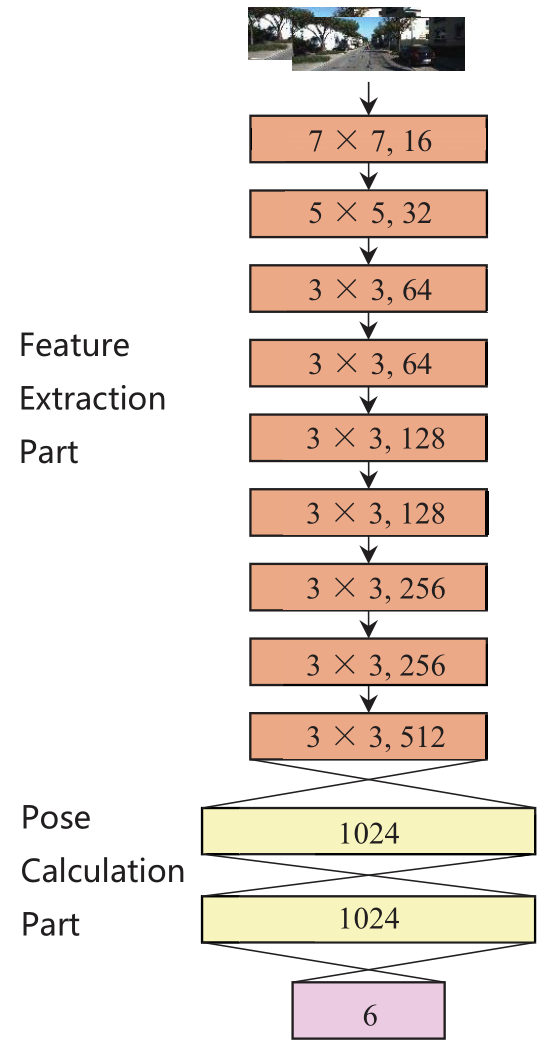
\includegraphics[width=0.32\textwidth]{./imgs/menet_structure.png}
    \end{center}
    \caption{MeNet model architecture.}
    \label{fig:menet-structure}
\end{figure}

In order to train the model, we use a loss function that consists in the weighted composition of two Mean Square Errors (MSE) computed separately on positions and quaternions:
\begin{equation}
    Loss(w) = \frac{1}{N} \sum\limits_{i=1}^N \norm{P^i - \hat{P}^i}^2_2 + \alpha\norm{Q^i - \hat{Q}^i}^2_2
    \label{eq:menet-loss}
\end{equation}
where $P$, $\hat{P}$, $Q$, $\hat{Q}$, and $\alpha$ are the ground truth position vector, the estimated position vector, the ground truth quaternions, the estimated quaternions, and the weight for balancing the displacement error and the rotation angle error.

\subsection{PoseNet}
Since the results given by RPE deep learning solutions are not very promising due to the lack of generalization and to cumulative errors in the estimations, from now on we are going to consider only models strictly developed for APE.
In this sense, the first one we present is the PoseNet model~\cite{9348762}.
As shown in \cref{fig:mapnet-posenet-structure}, just like the MeNet model, the PoseNet is made up by two components:
\begin{itemize}
    \item feature extraction through a sequence of convolutional layers. This component has been named internally also as \emph{backend};
    \item pose regression on the extracted features using linear layers.
\end{itemize}

\begin{figure}[htbp]
    \begin{center}
        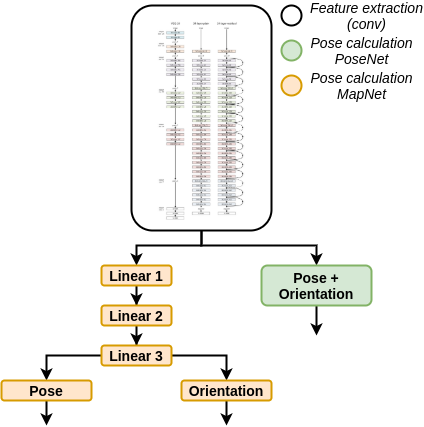
\includegraphics[width=0.32\textwidth]{./imgs/mapnet_posenet_structure.png}
    \end{center}
    \caption{PoseNet and MapNet model architecture.}
    \label{fig:mapnet-posenet-structure}
\end{figure}

This model architecture is actually pretty convenient, since it can use pre-trained deep convolutional networks, through the transfer learning approach. In most of the cases, this kind of models are trained on the ImageNet dataset \cite{imagenet}, which counts almost 3.2 millions real-world images: this offer good generalization capabilities for the feature extraction task.
It is important to notice that these models have been developed to work on the ImageNet dataset, which consists of RGB 224x224 pixels images: for this reason, any PoseNet input must have the same shape. 
Some examples of state-of-the-art backend models that have been considered are: GoogLeNet~\cite{googlenet}, ResNet~\cite{resnet}, and EfficientNet-B7~\cite{efficientnet}. \Cref{tab:backend-performance-imagenet} shows the accuracy over the k=(1, 5) top predictions for the used backends on the ImageNet dataset.

\begin{table}[htbp]
    \caption{Backends performance in ImageNet}
    \begin{center}
        \begin{tabular}{lrrr}
            \toprule
            Model           & Acc@1           & Acc@5           & Parameters      \\
            \midrule
            GoogLeNet       & 69.778          & 89.530          & $\sim$ 7,000,000\\
            ResNet-18       & 69.758          & 89.078          & 11,180,103      \\
            ResNet-34       & 73.314          & 91.420          & 21,288,263      \\
            ResNet-50       & 76.130          & 92.862          & 23,522,375      \\
            ResNet-152      & 78.312          & 94.046          & 58,158,151      \\
            EfficientNet-B7 & \textbf{84.122} & \textbf{96.908} & 63,804,887      \\
            \bottomrule
        \end{tabular}
        \label{tab:backend-performance-imagenet}
    \end{center}
\end{table}

Since ImageNet pre-trained models are used for classification purposes, we need to remove the last classification-related layers, and use only the convolutional ones for feature extraction. This gives us the opportunity to insert in the PoseNet a feature extraction mechanism on real-world images with minimum effort: training by scratch such models would require a huge amount of computational power.

Moreover, to train the PoseNet we adopt the weighted loss described in \cref{eq:menet-loss}, also used in the MeNet model.

\subsection{MapNet}
The MapNet model for APE represents an evolution of the PoseNet model: in fact, the model architecture remains actually the same, as shown in \cref{fig:mapnet-posenet-structure}. While even in this case the original model has a single linear layer, we introduce a sequence of them, each followed by the RELU activation function. This enables the model to learn more complex scenarios fitting better the data distribution.

Another difference with respect to the PoseNet is the loss function used to train the model. In this case, the errors on the prediction of absolute poses are not the only ones which are penalized: in fact, also errors in the relative poses are taken in consideration. To be able to penalize also relative errors, during the training process the model receives as input a batch of \texttt{step} ($s$) sorted frames, that are separated by \texttt{skip} ($k$) frames in the original video.
\Cref{eq:mapnet-loss} describes the MapNet loss as a mixture of absolute and relative errors regularized by the $\alpha$ hyperparameter: 

\small
\begin{equation}
    L_\mathcal{D}(\Theta) = \sum\limits_{i=1}^{|\mathcal{D}|} h([\hat{P}^i \hat{Q}^i], [P^i Q^i]) + \alpha\sum\limits_{i,j=1, i\neq j}^{|\mathcal{D}|} h([\hat{P}^{ij} \hat{Q}^{ij}], [P^{ij} Q^{ij}])
    \label{eq:mapnet-loss}
\end{equation}
\normalsize
where $[P^{ij} Q^{ij}]$ is the relative camera pose between pose predictions $[P^i Q^i]$ and $[P^j Q^j]$ for images $I^i$ and $I^j$.
$h(\cdot)$ is a function to measure the distance between the predicted camera pose $\hat{P}$ and the ground truth camera pose $P$, defined as:
\small
\begin{equation}
    h([\hat{P}^i \hat{Q}^i], [P^i Q^i]) = \norm{\hat{P}^i-P^i}_1 e^{-\beta} + \beta + \norm{\hat{Q}^i-Q^i}_1 e^{-\gamma} + \gamma
    \label{eq:mapnet-loss-h}
\end{equation}
\normalsize
where $\beta$ and $\gamma$ are the weights that balance the position loss and rotation loss. Both the parameters can be learned as well during the training procedure. $(I^i, I^j)$ are image pairs within each tuple of $s$ images sampled with a gap of $k$ frames from $\mathcal{D}$.
